Pour des raisons de lisibilité, nous avons réalisé une analyse descendante globale, puis nous l'avons découpé en sous-analyses descendantes pour pouvoir afficher les entrées sorties clairement.

\begin{figure}[H]
	\centering 
	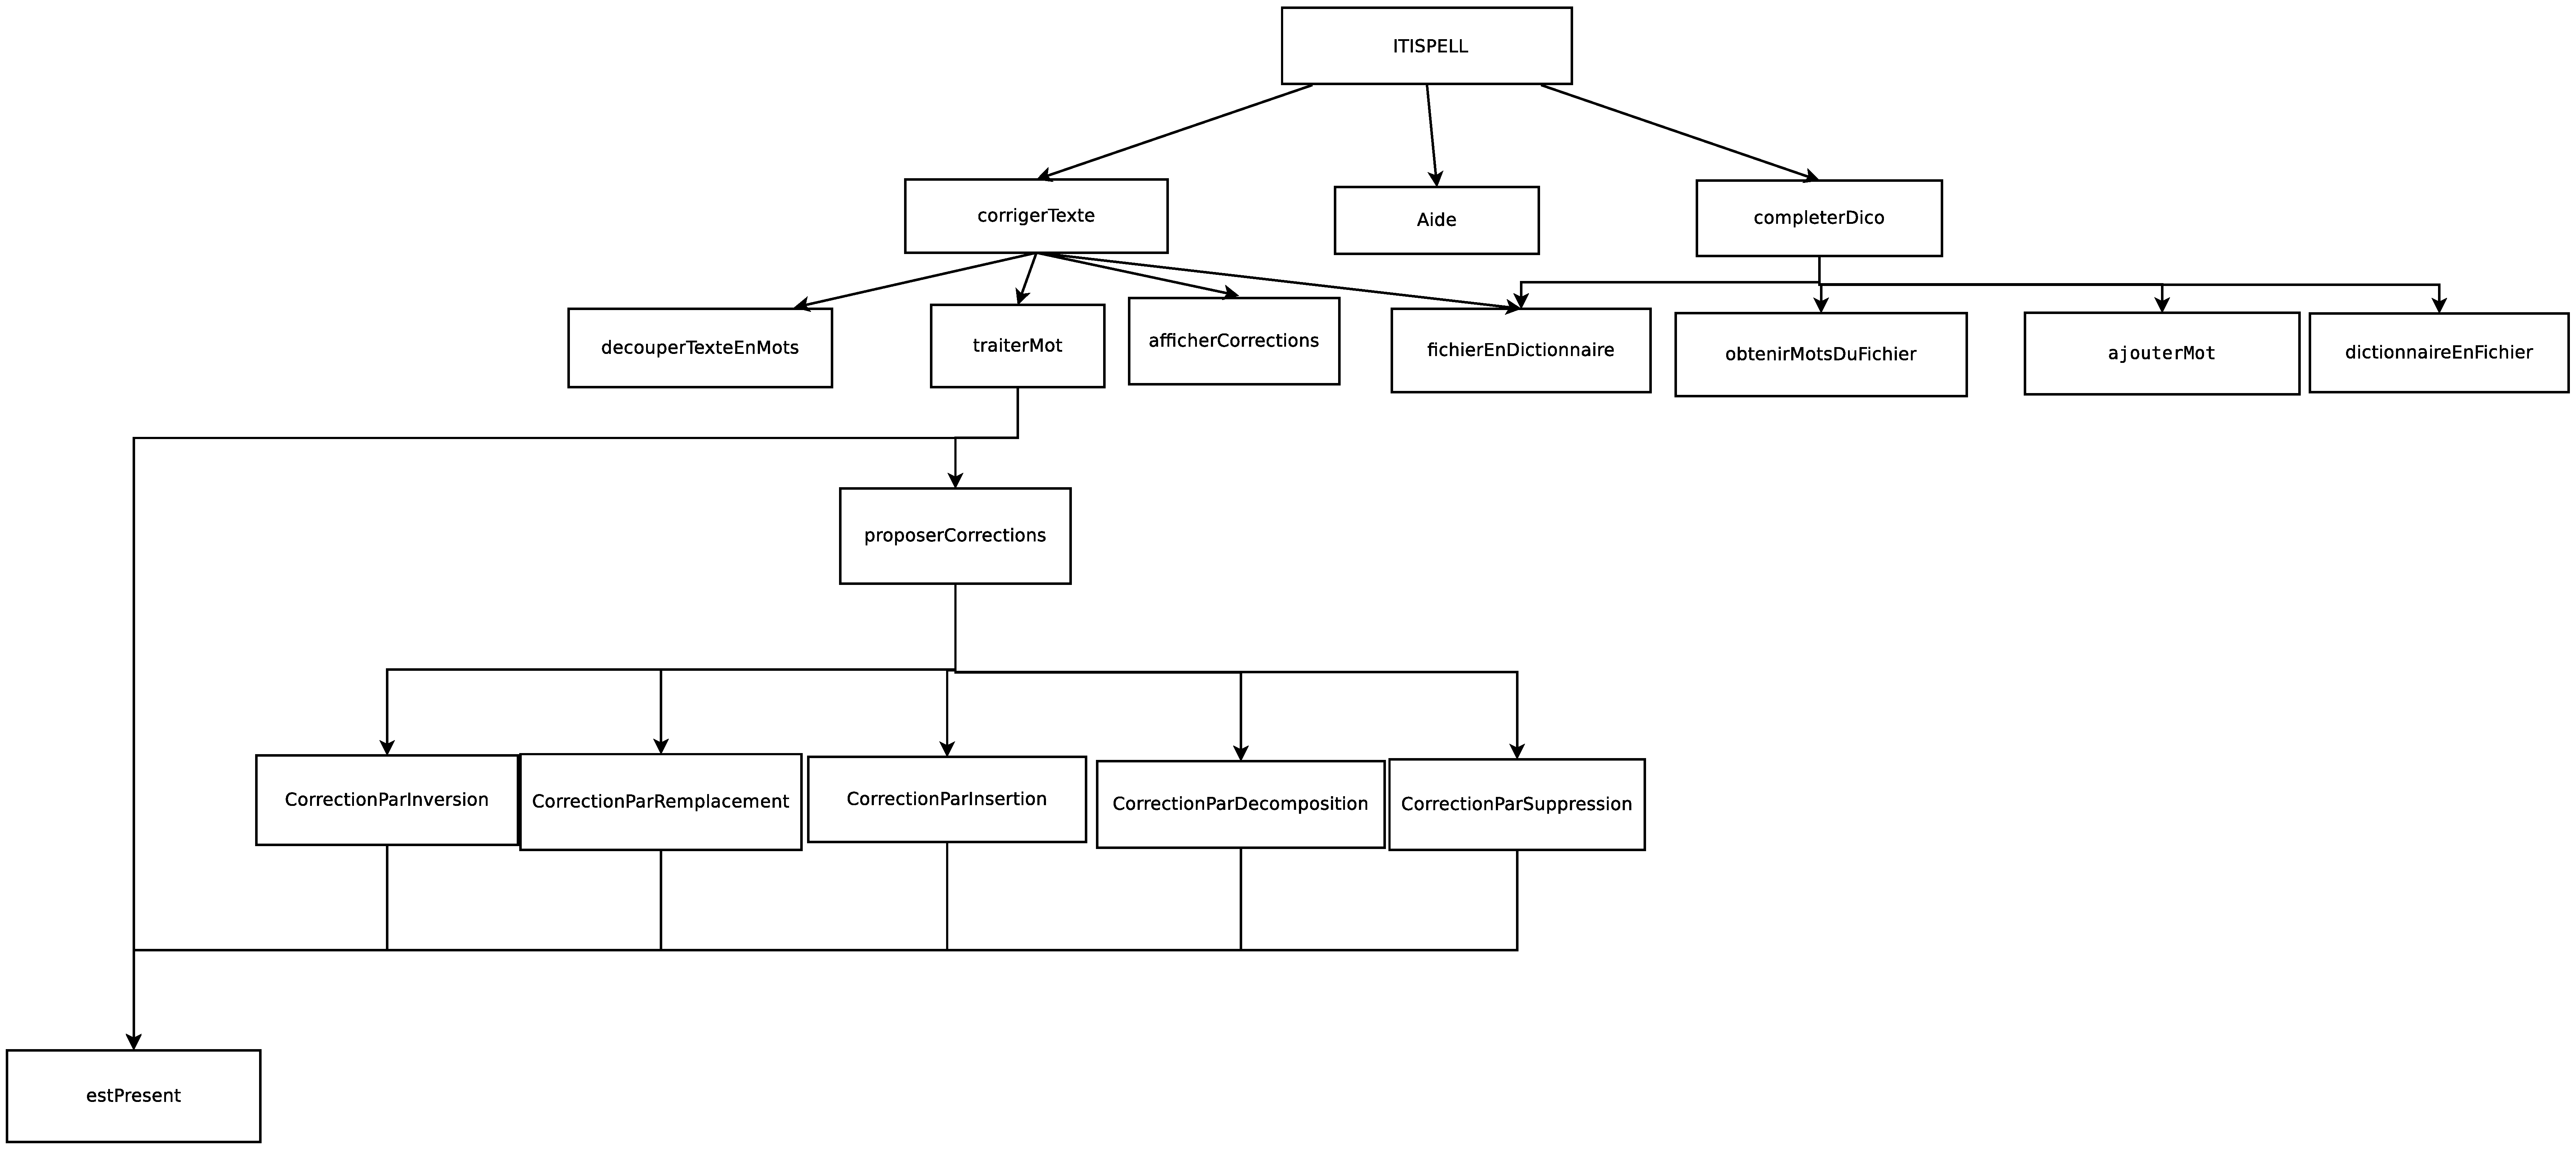
\includegraphics[width=\textwidth]{images/AD_globale.eps}
	\caption{Analyse descendante globale du projet}
	\label{fig:ADglobale}
\end{figure}
\begin{figure}[H]
	\centering 
	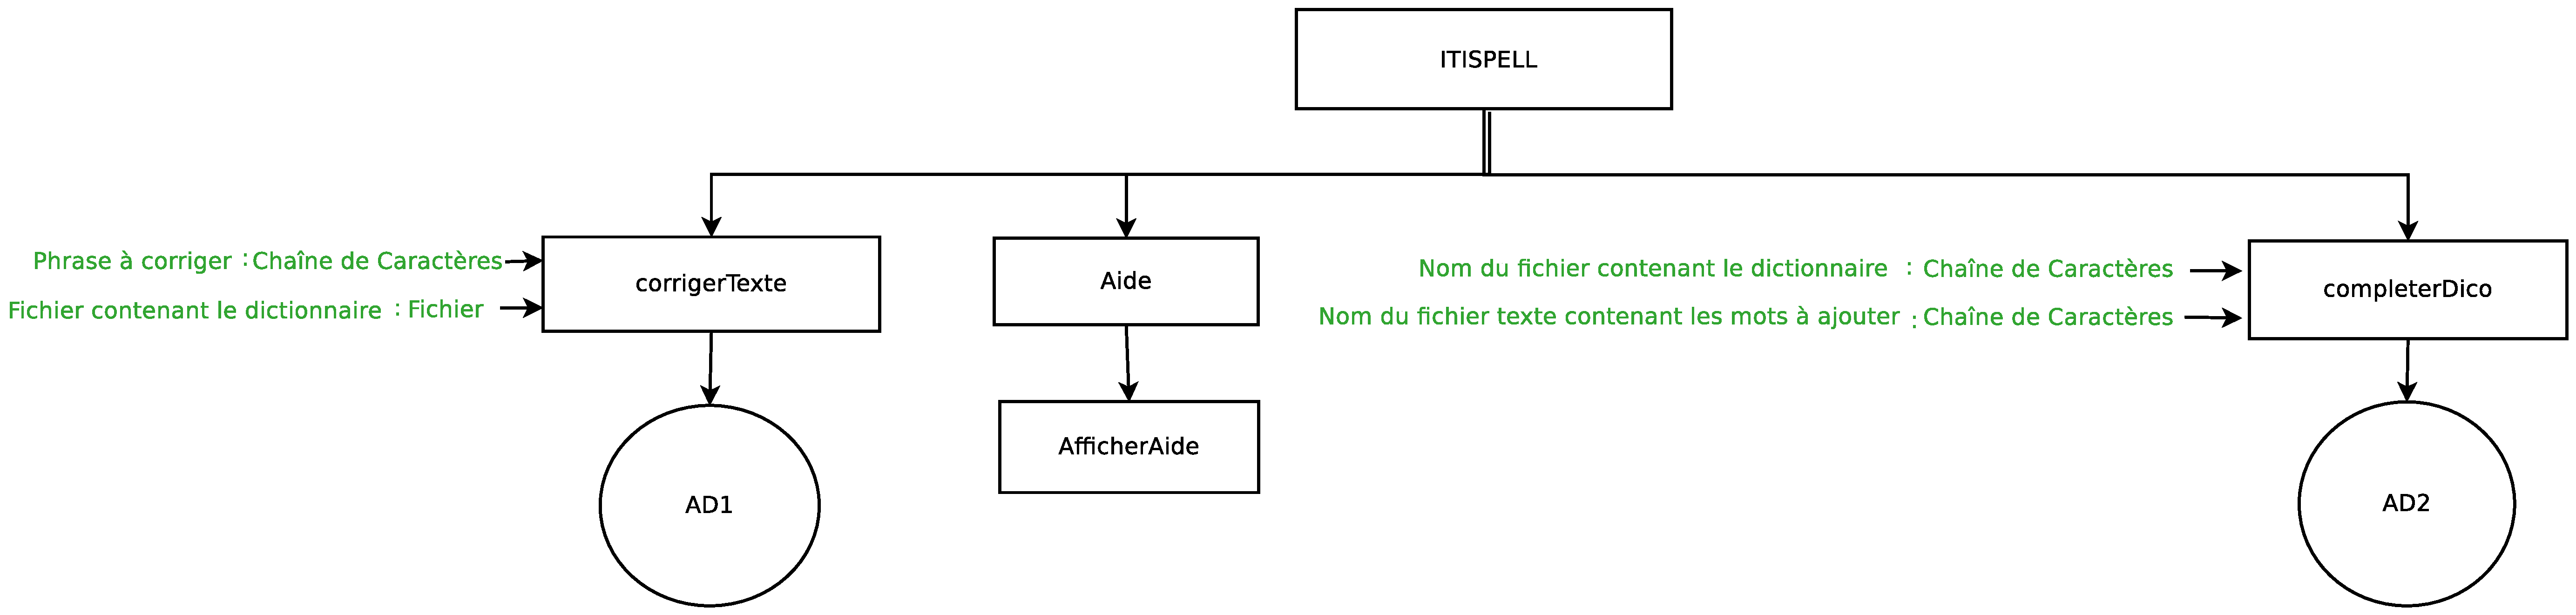
\includegraphics[width=\textwidth, angle=90, scale = 1.3]{images/AD0.eps}
	\caption{Analyse descendante simplifiée (AD0)}
	\label{fig:AD0}
\end{figure}
\begin{figure}[H]
	\centering 
	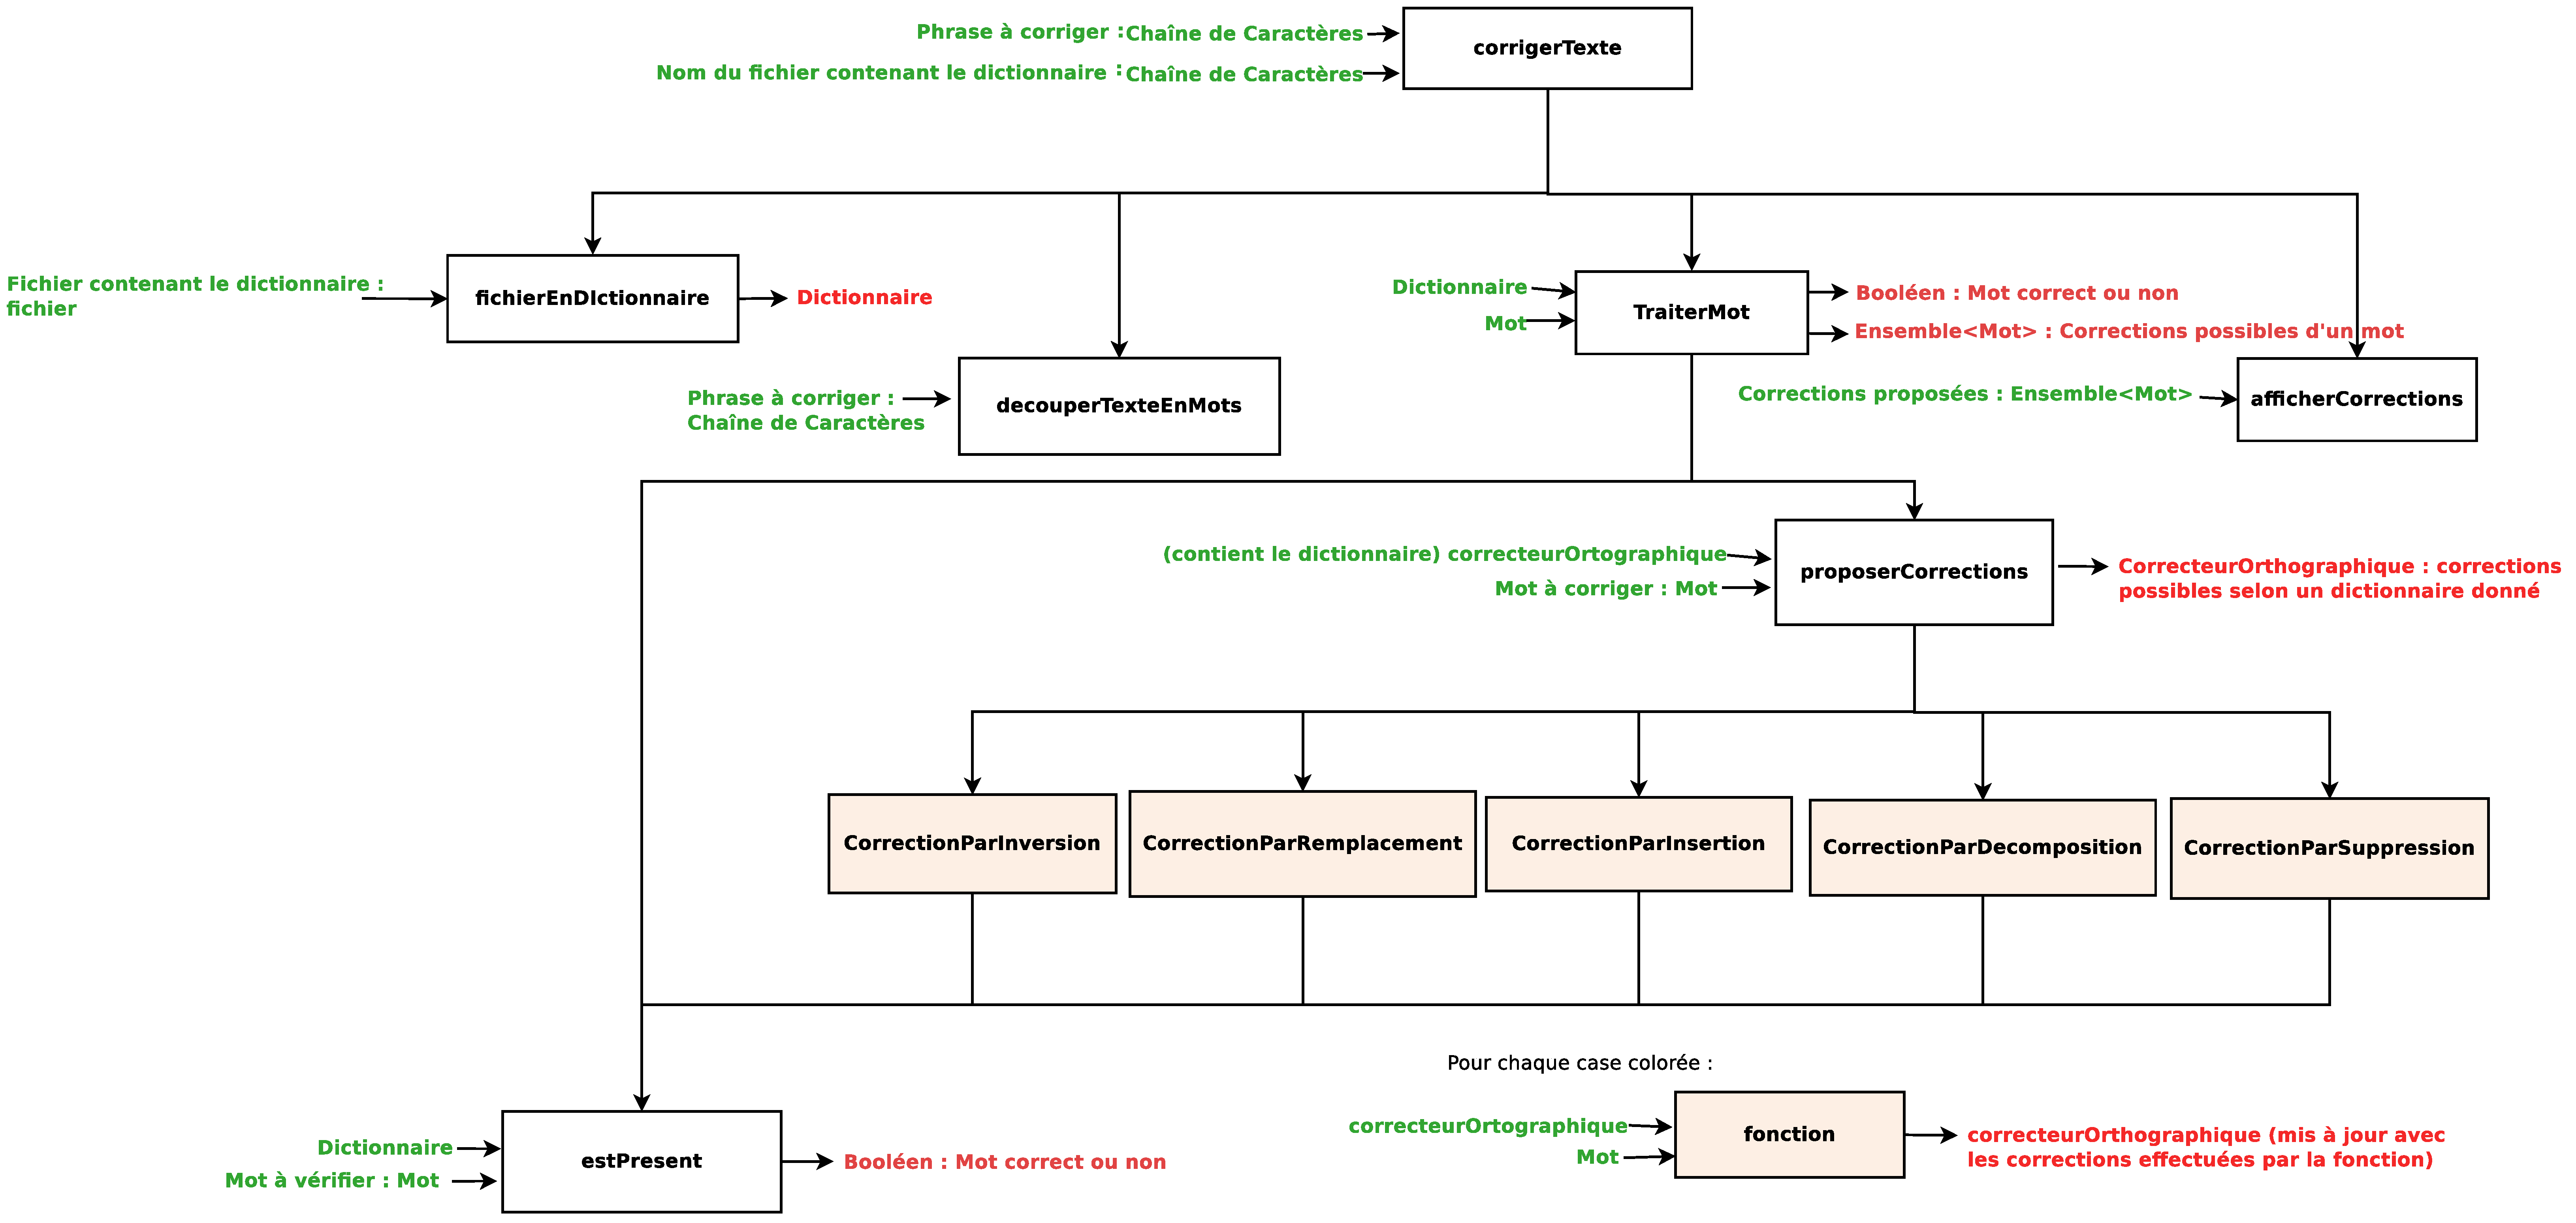
\includegraphics[width=\textwidth, angle=90, scale = 1.3]{images/AD1.eps}
	\caption{Analyse descendante de la partie correction (AD1)}
	\label{fig:AD1}
\end{figure}
\begin{figure}[H]
	\centering 
	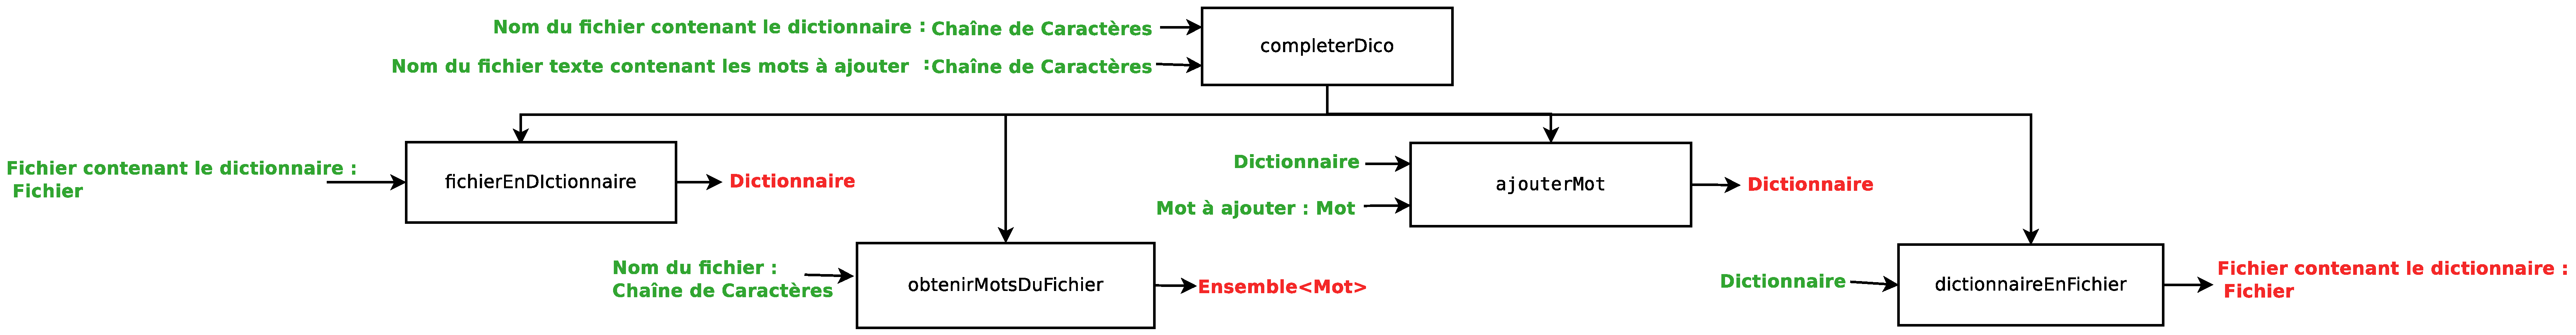
\includegraphics[width=\textwidth, angle=90, scale = 1.3]{images/AD2.eps}
	\caption{Analyse descendante de la partie complétion (AD2)}
	\label{fig:AD2}
\end{figure}